%% Author_tex.tex
%% V1.0
%% 2012/13/12
%% developed by Techset
%%
%% This file describes the coding for rsproca.cls

\documentclass[]{rsos}%%%%where rsos is the template name

\usepackage{lineno}
\linenumbers

\usepackage[T1]{fontenc}
\usepackage[utf8]{inputenc}


%%%% *** Do not adjust lengths that control margins, column widths, etc. ***

%%%%%%%%%%% Defining Enunciations  %%%%%%%%%%%
\newtheorem{theorem}{\bf Theorem}[section]
\newtheorem{condition}{\bf Condition}[section]
\newtheorem{corollary}{\bf Corollary}[section]
%%%%%%%%%%%%%%%%%%%%%%%%%%%%%%%%%%%%%%%%%%%%%%%

\begin{document}

%%%% Article title to be placed here
\title{Evolutionary simulations of \emph{Z}-linked suppression gene drives}

\author{
Luke Holman$^{1}$}

\address{
  $^{1}$School of BioSciences, The University of Melbourne, Victoria 3010,
Australia.}
%%%% Subject entries to be placed here %%%%
\subject{
Evolutionary biology,
Theoretical modelling,
Gene drives}

%%%% Keyword entries to be placed here %%%%
\keywords{
Sex chromosomes,
Gene drives,
Population control,
Schistosomiasis,
Selfish genes}

%%%% Insert corresponding author and its email address}
\corres{
  L. Holman\\
  e-mail: \href{mailto:luke.holman@unimelb.edu.au}{\nolinkurl{luke.holman@unimelb.edu.au}}
}

%%%% Abstract text to be placed here %%%%%%%%%%%%
\begin{abstract}
Synthetic gene drives may soon be used to suppress or eliminate
populations of disease vectors, pathogens, invasive species, and pests.
Recent proposals have suggested that one could use a gene drive carried
on the \emph{Z} chromosome to create male-biased sex ratios in species
with \emph{ZW} sex determination, which include Lepidopteran
agricultural pests and parasitic trematodes. For example, a
\emph{Z}-linked `\emph{W}-shredder' might exhibit gene drive by cleaving
the \emph{W} chromosome and thereby causing carrier females to produce
only sons. Here I use eco-evolutionary simulations to evaluate
\emph{W}-shredders and other hypothesised \emph{Z}-linked gene drives,
and to produce recommendations regarding their design and use. I
conclude that \emph{W}-shredders are likely to be highly effective at
eradicating populations provided that resistance cannot evolve, but it
may be hard to confine the drive allele to particular populations or
geographic regions.
\end{abstract}
%%%%%%%%%%%%%%%%%%%%%%%%%%%

%% Some pieces required from the pandoc template
\providecommand{\tightlist}{%
  \setlength{\itemsep}{0pt}\setlength{\parskip}{0pt}}
\providecommand{\EndFirstPage}{%
}

\maketitle

\hypertarget{introduction}{%
\section{Introduction}\label{introduction}}

Developments in genetic engineering will soon make it feasible to alter
or eliminate populations of disease vectors, pathogens, agricultural
pests, and invasive species using `gene drives'
\citep{gantz2015hi, hammond2016cr, wang2016cr, prowse2017do, kyrou2018cr, noble2018cu}.
Gene drives cause particular alleles (usually transgenes) to propagate
through populations via a range of mechanisms, which include gene
conversion, poison-antidote systems, segregation distortion, and genetic
incompatibility \citep{lindholm2016ec, champer2016ch, oberhofer2019cl}.
For example, CRISPR-Cas9 gene editing can be used to create a transgenic
insertion that is transmitted to almost 100\% of the offspring of
heterozygous individuals instead of the usual 50\%; this type of gene
drive functions by inducing a double-stranded DNA break at the
homologous wild type locus, which is then repaired using the transgene
as a template. Gene drives are often categorised into two types:
replacement drives, which aim to spread a human-beneficial allele
throughout a population (e.g.~a mosquito allele that interferes with the
tranmission of malaria \citep{gantz2015hi, marshall2015gene}), and
suppression drives, which reduce the size of a population (potentially
to extinction). Suppression drives typically work by using non-Mendelian
inheritance to spread alleles that cause lethality or sterility
\citep{hammond2016cr, kyrou2018cr, maselko2018ge}, or skew the offspring
sex ratio -- typically towards males
\citep{windbichler2008ta, galizi2014sy, beaghton2017ve, burt2018se, papathanos2018re}.

Recent theoretical papers have investigated the feasibility, efficacy,
and potential negative consequencies of various types of gene drives.
For example, Noble et al. \citep{noble2018cu} used models to show that
the basic version of a CRISPR-Cas9 gene drive might be highly invasive
and could rapidly spread to fixation across whole species, which is
often an undesirable outcome. Conversely, other models have concluded
that gene drives are likely to fail if populations can evolve resistance
to their effects \citep{drury2017cr, unckless2017ev}. The issue of
resistance is compounded because the standard implementation of
CRISPR-Cas9 gene drive (but perhaps not updated versions;
\citep{esvelt2014em, unckless2017ev, prowse2017do, kyrou2018cr}) tends
to create its own resistance alleles, e.g.~when the double-stranded
break induced by Cas9 is repaired using an alternative DNA repair
pathway (non-homologous end joining; NHEJ) instead of homology-directed
repair
\citep{gantz2015mu, gantz2015hi, hammond2016cr, wang2016cr, unckless2017ev}.
Given the potential safety, ethical, and sociopolitical concerns
surrounding gene drives, some models have focused on gene drives that
would go extinct after a time
\citep{min2017da, burt2018se, noble2019da}, would stay confined to
particular populations \citep{maselko2018ge, noble2019da}, and/or could
be reversed once they have spread \citep{vella2017ev}.

Here, I focus on the evolutionary dynamics of \emph{Z}-linked
suppression gene drives. The simulation is inspired by proposals for
various types of \emph{Z}-linked gene drives by Kevin Esvelt and
colleagues, as well as ongoing efforts to develop these \emph{Z} drives
(see \href{}{www.sculptingevolution.org}; at the time of writing, these
ideas have not been published elsewhere). Various \emph{Z}-linked
suppression drives proposed by Esvelt and colleagues are shown
schematically in Figure 1. Depending on its design, mode of action and
the biology of the target species, \emph{Z} chromosomes carrying the
drive allele (denoted \emph{Z*}) might enjoy a transmission advantage in
\emph{Z*W} females (Figure 1B, and perhaps also 1C), and optionally also
in \emph{Z*Z} males. Esvelt et al.~focus on using \emph{Z} drives to
control the \emph{Schistosoma} trematodes responsible for
schistosomiasis, though \emph{Z} drives could theoretically be used to
control any organism with female-heterogametic sex determination, such
as Lepidopteran agricultural pests or even invasive populations of
birds.

A \emph{Z}-linked gene drive could suppress populations by biasing
gametogenesis in females, for example by inducing double-stranded DNA
breaks in the \emph{W} chromosome in order to inactivate it; such a gene
drive would be a `\emph{W}-shredder', analagous to the \emph{X}- and
\emph{Y}-shredders under development for \emph{XY} species
\citep{windbichler2008ta, north2013mo, galizi2014sy, burt2018se, papathanos2018re, prowse2019}.
Females carrying the gene drive would thus produce relatively few viable
\emph{W}-bearing eggs, and therefore produce mainly drive-carrying sons.
Esvelt et al.~point out that the evolutionary dynamics of the drive will
depend on the fitness of drive carriers relative to wild types, the
timing of \emph{W}-shredding (e.g.~in germ cells, ova, or zygotes), and
the ecology of the target species. For example, some \emph{W}-shredder
designs might allow drive females to produce roughly the same number of
(mostly-male) offspring as a wild-type female provided that the \emph{W}
chromosome is destroyed early enough in oogenesis/development that the
lost daughters can be replaced by sons (Figure 1B). Alternatively,
drive-carrying females might produce half the number of offspring (or
less), e.g.~if the drive works by destroying all ova or offspring that
carry a \emph{W} chromosome, and this loss is not compensated by reduced
competition on the surviving offspring. Esvelt et al.~also proposed that
one could suppress populations using a \emph{Z}-linked locus that caused
sterility or lethality in females, either by shredding the \emph{W} in
somatic tissues, or by spreading some other allele that harms females
only. If this female-harming allele were capable of gene drive in males,
or were continually released into the wild, it could perhaps reach high
enough frequencies to suppress the population. The \emph{W}-shredder
could be designed to also cause gene drive in males. Male gene drive
could be accomplished using `standard' CRISPR-Cas9 gene conversion,
whereby the driving \emph{Z} allele would convert the wild type locus
using homing endonuclease activity followed by homology-directed repair,
causing heterozygous males to produce mostly drive-carrying sperm.
Esvelt et al.~note that male gene drive might not be necessary, since a
\emph{Z}-linked locus that prevents transmission of the \emph{W} may
already enjoy a transmission advantage (Figures 1B-1C).

Here, I present an evolutionary simulation that can accommodate all of
these hypothetical \emph{Z}-linked drives. I aimed to test which
properties of the gene drive and the ecology of the target species are
critical to determining the likelihood and speed of extinction. For
example, the gene drive will presumably spread faster if it can bias
transmission in both sexes, but perhaps a simpler female-only drive
would be perfectly adequate. Also, since the population will become more
male-biased as the gene drive invades, there will be eco-evo feedback
that might affect the evolutionary outcome in non-intuitive ways. For
example, the altered sex ratio might intensify the fitness advantage
accruing to any resistant \emph{W} chromosomes or autosomal modifiers
that prevent \emph{W}-shredding (due to Fisherian selection for an even
sex ratio; \citep{holman2015co}), relative to that observed in earlier
models focusing on gene drives carried on autosomes
\citep{unckless2017ev, drury2017cr}. Moreover, the change in sex ratio
could affect the ecology and evolution of the population, particularly
if males and females contribute differentially to density-dependent
population growth \citep{rankin2007ma, li2019int}, or have different
dispersal rates \citep{li2019sex}. The model incorporates the
possibility that \emph{Z}-linked resistant-to-drive alleles are
sometimes created by NHEJ in heterozygote males, to test whether
resistance is just as problematic as for autosomal drives
\citep{gantz2015mu, gantz2015hi, hammond2016cr, wang2016cr, unckless2017ev}.

\hypertarget{methods}{%
\section{Methods}\label{methods}}

\hypertarget{overview}{%
\subsection{Overview}\label{overview}}

I model a finite population of dioecious diploids with \emph{ZW} sex
determination, living in \(j\) discrete habitat patches that are
arranged linearly in a ring. The model considers the demography and
evolution of a population into which \(n_{release}\) males carrying a
\emph{Z}-linked gene drive allele (\emph{Z*}) are released. The drive
allele causes either \emph{W}-shredding or sterility in females, and
optionally also causes gene drive in heterozygous males (e.g.~via gene
conversion). Each generation proceeds as follows: birth, dispersal
between patches, breeding within patches, and death of the parental
generation. The species has 3 loci with 2-3 alleles each, some of which
potentially show non-Mendelian inheritance. The equilibrium population
size was roughly 10,000 in all simulations upon release of the gene
drive, and the main outcomes of interest are the likelihood and speed of
extinction. The model is a stochastic individual-based simulation
written in R 3.4.0; it was run on the Spartan cluster at the University
of Melbourne.

\hypertarget{loci-and-alleles}{%
\subsection{Loci and alleles}\label{loci-and-alleles}}

Each male in the simulation carries one \emph{Z}-linked locus and two
autosomal loci, each with two alleles. Each female carries a single
allele at the \emph{Z}-linked locus plus a \emph{W} chromosome, as well
as two alleles at both of the autosomal loci.

There are three possible \emph{Z}-linked alleles: a gene drive allele
(\emph{Z*}), a wild-type allele (\(Z^+\)) that is vulnerable to gene
drive in \emph{Z*}\(Z^+\) males, and a resistant allele (\(Z^r\)) that
is immune to gene drive in \emph{Z*}\(Z^r\) males. Similarly, there are
two possible types of \emph{W} chromosomes: a wild-type \emph{W}
chromosome (\(W^+\)) that is vulnerable to gene drive by the \emph{Z*}
allele, and a resistant \emph{W} chromosome (\(W^r\)) that is immune to
gene drive.

The two autosomal loci, denoted \emph{A/a} and \emph{B/b}, control
immunity to \emph{W}-shredding and gene conversion respectively.
\emph{A/a} and \emph{B/b} are `trans-acting' resistance loci, since they
are at a different locus (indeed, a different chromosome) to the gene
drive allele, in contrast to the `cis-acting' resistance conferred by
the \(Z^r\) and \(W^r\) alleles. The \emph{A} allele is dominant and
confers immunity to \emph{Z}-linked gene drive (e.g. \emph{W}-shredding)
in females. The \emph{B} allele is dominant and confers immunity to
\emph{Z}-linked gene drive (e.g.~gene conversion) in males.

\hypertarget{calculating-fitness}{%
\subsection{Calculating fitness}\label{calculating-fitness}}

Individuals with no \emph{Z*} alleles have an intrinsic fitness of \(w\)
= 1, while other genotypes have \(0 \le w \le 1\). The fecundity of
females carrying \emph{Z*} is reduced by a factor \(1 - c_f\). Small
\(c_f\) implies minimal costs (e.g.~because mothers replace lost
gametes/offspring and/or sib-sib competition is intense), \(c_f = 0.5\)
could represent the case where all daughters die and are not replaced,
and \(c_f = 1\) means that females carrying \emph{Z*} are completely
sterile. Setting \(c_f = 1\) allows simulation of a female-sterilising
\emph{Z}-linked drive. Similarly, the fitness of males carrying
\emph{Z*} is reduced by a factor \(1 - c_m\); male fitness determines
mating success (see below). For simplicity, I assume that the resistance
alleles \(W^r\), \(Z^r\), \emph{A} and \emph{B} are cost-free. Also, the
costs of \emph{Z*} to males were assumed to be dominant, such that
\emph{Z*}\(Z^+\) males and \emph{Z*Z*} males had equal fitness.

\hypertarget{gamete-production-and-gene-drive}{%
\subsection{Gamete production and gene
drive}\label{gamete-production-and-gene-drive}}

I assume that the \emph{A/a} and \emph{B/b} loci segregate independently
during meiosis and display standard Mendelian inheritance. Inheritance
of the sex chromosomes is also Mendelian except for certain genotypes
carrying one \emph{Z*} allele.

Firstly, \emph{Z*}\(W^+\)\emph{aaBB}, \emph{Z*}\(W^+\)\emph{aaBb}, and
\emph{Z*}\(W^+\)\emph{aabb} females produce a fraction
\(\frac{1}{2}(1 + p_{shred})\) of \emph{Z}-bearing gametes and
\(\frac{1}{2}(1 - p_{shred})\) \emph{W}-bearing gametes. Therefore,
these three female genotypes produce \textgreater{}50\% sons when
\(p_{shred} > 0\), due to the shortage of \emph{W} chromosomes in their
gametes. The gamete frequencies of \emph{Z*}\(W^r\) females, or of
females carrying at least one \emph{A} allele, conform to the standard
Mendelian expectations due to resistance.

Secondly, \emph{Z*}\(Z^+\)\emph{AAbb}, \emph{Z*}\(Z^+\)\emph{Aabb}, and
\emph{Z*}\(Z^+\)\emph{aabb} males produce a fraction
\(\frac{1}{2}(1 + p_{conv} - p_{conv} p_{nhej})\) of gametes carrying
the \emph{Z*} allele, \(\frac{1}{2}(1 - p_{conv})\) gametes carrying the
\(Z^+\) allele, and \(\frac{1}{2}(p_{conv} p_{nhej}))\) gametes carrying
the \(Z^r\) allele. Thus, gene conversion occurs in males if
\(p_{conv} > 0\), meaning that the \emph{Z*} allele is over-represented
in the gametes of these three male genotypes. The parameter \(p_{nhej}\)
represents the creation of resistance alleles via non-homologous end
joining, in which the gene drive fails to copy itself to the homologous
chromosome, and instead induces an indel mutation that creates a
resistant allele. The gamete frequencies of \emph{Z*}\(Z^r\) males, or
of males carrying at least one \emph{B} allele, conform to the standard
Mendelian expectations due to resistance.

\hypertarget{calculating-female-fecundity}{%
\subsection{Calculating female
fecundity}\label{calculating-female-fecundity}}

In the breeding phase of the lifecycle, the simulation first determines
the number of offspring produced by each female. The expected fecundity
of female \(i\) (\(F_i\)) is affected by three factors: the female's
genotype, the density of males and females in the local patch and/or in
the full population, and some global parameters in the model, as
follows:

\begin{equation}
\tag{1}
F_i = (1 + w_i r(1 - (D_i / K) ^ \alpha))
\end{equation}

where \(D_i\) is the `density' experienced by female \(i\), \(w_i\) is
her fitness, \(K\) is the carrying capacity, and \(r\) and \(\alpha\)
are constants that control the maximum possible fecundity and the shape
of density-dependence respectively (function from \citep{fowler1981de}).

To ensure that the simulation captures various possible types of life
history and ecology, I calculated density \(D_i\) in various ways in
different simulation runs. First, I define the global density \(d_g\),
which acts equally on every female in every patch, as

\begin{equation}
\tag{2}
d_g = \sum_{i=1}^{N_f} w_i + \delta N_m
\end{equation}

where \(N_f\) and \(N_m\) are the numbers of females and males across
all patches, the first term is the summed fitnesses of all these
females, and \(\delta\) is a constant (range: \(0-\infty\)) that scales
the effect of each male on \(d_g\) relative to a female with fitness
\(w_i = 1\). This formulation means that females with high relative
fitness (i.e.~fecundity) have a stronger effect on the global density
than do low-fitness females. I also assume that each male contributes a
fixed amount to the global density, irrespective of his genotype/fitness
(since I assume that male fitness only affects male mating success; see
below). The parameter \(\delta\) represents sex differences in
ecological niche use and behaviour. For example, we might expect
\(\delta<1\) in species where males and females utilise very different
environmental niches, or \(\delta>1\) in species where males are harmful
to females.

Second, I define the local density \(d_j\) experienced by every female
in patch \(j\), as

\begin{equation}
\tag{3}
d_j = \sum_{i=1}^{n_{f,j}} w_i + \delta n_{m,j}
\end{equation}

where \(n_{f,j}\) and \(n_{m,j}\) are the numbers of females and males
in patch \(j\). As before, this formulation means that \(d_j\) depends
on the summed fitnesses of the females in the patch, as well as the
number of males (scaled by the constant \(\delta\)).

Finally, the overall density experienced by female \(i\) in patch \(j\)
(\(D_i\)) is a weighted sum of the global and local densities given by
\(D_i = \psi d_g + (1 - \psi)d_j\), where the parameter \(\psi\) weights
the importance of global and local density to female fecundity. When
\(\psi = 0\), only local density matters and selection on females is
entirely `soft', while when \(\psi = 1\) only global density matters and
selection on females is completely `hard' (as in \citep{li2018ev}).
Intermediate values of \(\psi\) produce a mixture of hard and soft
selection on females.

After calculating the expected fecundity of each female (\(F_i\)), we
generate the realised fecundity of the female by randomly sampling from
a Poisson distribution with \(\lambda = F_i\) (allowing for stochastic
variation in fecundity between females with equal \(F_i\)). If the
resulting number of offspring exceeded the global carrying capacity
\(K\), the model randomly selects \(K\) surviving offspring.

\hypertarget{competition-between-males}{%
\subsection{Competition between males}\label{competition-between-males}}

After determining how many offspring each female produces, we determine
the fathers of each of these offspring. We assume that all breeding
occurs within patches, such that males only compete for
matings/fertilisations with males in the same patch. If the patch
contains \(k\) different male genotypes and there are
\(n_1, n_2, ... n_k\) males of each genotype, the probability that a
male of genotype \(k\) is the father of any given offspring is

\begin{equation}
\tag{4}
p_j = \frac{n_{k}w_k}{\sum_{i=1}^{k}n_{i}w_i}
\end{equation}

such that relatively common and/or high-fitness male genotypes are more
likely to sire offspring. This formulation means that both sexes
potentially reproduce with multiple partners.

\hypertarget{reproduction-mutation-and-dispersal}{%
\subsection{Reproduction, mutation and
dispersal}\label{reproduction-mutation-and-dispersal}}

After picking the parents, the model randomly generates each offspring's
genotype according to its parents' expected gamete (and thus zygote)
frequencies. Offspring are born in the same patch as their parents, and
the parental generation is replaced by the offspring generation.

When an offspring is created, each \(Z^+\) allele it carries has a
chance \(\mu_Z\) to mutate to a \(Z^r\) allele, and \emph{vice versa}
(i.e.~mutation in both directions is equally probable). Similarly, each
\emph{W+} allele has a chance \(\mu_W\) to mutate to a \(W^r\) allele,
and \emph{vice versa}.

Female and male offspring disperse to another patch with probabilities
\(x_f\) and \(x_m\) respectively. We model two types of dispersal, in
separate simulations: local dispersal, in which offspring move to one of
the two neighbouring patches with equal probability (recalling that the
patches are arranged in a ring), or global dispersal, in which
dispersing offspring can land in any of the other patches.

\hypertarget{one-compete-run-of-the-simulation}{%
\subsection{One compete run of the
simulation}\label{one-compete-run-of-the-simulation}}

The model first initialises a population of 10,000 individuals (the
carrying capacity, \(K\)) with low or zero frequencies of \(Z^r\),
\(W^r\), \emph{A} and \emph{B} alleles, higher frequencies of the wild
type \(Z^+\), \emph{W+}, \emph{a}, and \emph{b} alleles, and zero
\emph{Z*} gene drive alleles. It then runs 50 generations of burn-in to
allow the population to reach demographic and genotypic equilibrium.
Next, \(n_{release}\) males with the genotype \emph{Z*Z*aabb} are added
to the population just before fathers are selected, representing the
release into the wild of a laboratory-reared strain homozygous for the
driving \emph{Z}. In some simulations, all the \emph{Z*Z*aabb} males
were released in a single patch, while in others the \(n_{release}\)
males were randomly and evenly divided across all \(k\) patches. The
model continued until either A) the driving \emph{Z*} allele went
extinct, B) the population went extinct, C) the \(W^r\) chromosome went
to fixation (making population suppression impossible), D) the \emph{Z*}
allele fixed without causing extinction, or E) 1000 generations had
elapsed. The model recorded which of these five outcomes occurred, as
well as the allele frequencies, population size, and sex ratio at each
generation.

\hypertarget{investigating-the-parameter-space}{%
\subsection{Investigating the parameter
space}\label{investigating-the-parameter-space}}

For each of the parameters in Table 1, I selected two or more possible
parameter values (e.g.~high versus low rates of \emph{W}-shredding
\(p_{shred}\); many versus few patches \(k\)). I then ran the model once
for all possible combinations of these parameter values (n = 6,000,000
model runs). The aim was to measure the effect of each parameter across
various assumptions for the other parameters, as well as to investigate
all 2-way interactions between the parameters. To gauge the relative
importance of the various features of the \emph{Z*} allele and the
species' ecology to the extinction probability, I fit a binomial
generalised linear model (GLM) with extinction as the dependent
variable, and all the model parameters and their 2-way interactions as
predictors. The predictors were scaled and centred before running the
GLM, allowing for a meaningful ranking of the predictors by their
absolute effects on extinction.

\hypertarget{results}{%
\section{Results}\label{results}}

\hypertarget{three-illustrative-simulation-runs}{%
\subsection{Three illustrative simulation
runs}\label{three-illustrative-simulation-runs}}

Figure 2 shows three contrasting simulation runs. In Figure 2A, the
release of 20 \emph{Z*Z*} males at generation 50 resulted in invasion of
the \emph{Z*} allele, causing rapid extinction due to a lack of females.
This simulation run assumed that the \emph{Z*} alleles causes perfect
\emph{W}-shredding (\(p_{shred} = 1\)), that \emph{Z*} has minimal
fitness costs, and there is no resistance to \emph{W}-shredding (Table
S3).

In Figure 2B, \emph{Z*} invaded but failed to cause extinction, even
though it was assumed that \(p_{shred} = 1\) and \emph{W}-shredding was
not resistable. However, this simulation did assume that individuals
carrying at least one \emph{Z*} allele paid heavy fitness costs
(\(c_f = 0.5\) and \(c_m = 0.2\)), and that there was no gene drive in
males (\(p_{conv} = 0\)). The assumptions \(p_{shred} = 1\) and
\(c_f = 0.5\) could imply that the \emph{W}-bearing eggs/offspring of
\emph{Z*W+} females are destroyed and not replaced, such that
\emph{W}-shredding increases the proportion but not the absolute number
of offspring that inherit the \emph{Z*} allele. Essentially \emph{Z*}
spreads via `spite' \citep{gardner2006sp}, in that it removes \emph{W}
chromosomes from the local population and thereby makes room for more
\emph{Z*} alleles, creating indirect fitness benefits. However, the net
fitness returns of the \emph{Z*} allele's `strategy' (i.e.~sacrificing
20\% fitness in males in order to remove \emph{W} chromosomes in
females) decline as females become rarer, halting the spread of
\emph{Z*}.

Lastly, Figure 2C shows a case where the invasion of \emph{Z*} was
reversed by the evolution of autosomal and \emph{Z}-linked resistance
alleles. Following the introduction of the \emph{Z*} allele, resistant
\(Z^r\) mutants were created via non-homologous end joining, and then
\(Z^r\) spread to fixation due to its immunity to gene conversion in
males. The autosomal resistance allele \emph{A} also spread; \emph{A}
confers resistance to \emph{W}-shredding and was initially present in
the population at 5\% frequency. The spread of \emph{A} caused the sex
ratio to revert to normal, preventing extinction, and \emph{Z*} went
extinct due to its direct fitness costs no longer being outweighed by
the benefits of \emph{W}-shredding and gene conversion. Incidentally,
the resistant allele \emph{A} was favoured over \emph{a} because the
male-biased population sex ratio created by \emph{Z*} favours the
production of daughters, and \emph{AA} and \emph{Aa} females produce
more daughters than \emph{aa} females in populations where \emph{Z*} is
present.

\hypertarget{effects-of-each-parameter-on-the-evolution-of-a-w-shredder}{%
\subsection{\texorpdfstring{Effects of each parameter on the evolution
of a
\emph{W}-shredder}{Effects of each parameter on the evolution of a W-shredder}}\label{effects-of-each-parameter-on-the-evolution-of-a-w-shredder}}

Figure 3 shows the effects of each model parameter, for models of a
\emph{Z}-linked \emph{W}-shredder that potentially also benefits from
gene drive in \emph{Z*Z} males. Figure 4 shows the importance of each
main effect and two-way interaction term to the extinction probability,
while Figure S1 shows the effect of each parameter on the number of
generations until extinction. Under favourable assumptions, extinction
occurred around 20 generations after releasing \emph{Z*}, though it
often took longer (Figure S1). Tables S1-S2 give the relative
frequencies of the various possible outcomes (e.g.~extinction of the
population, or loss of \emph{Z*}).

In Figure 3, the parameters are arranged in order of their importance to
extinction probability (see also Figure 4). By far the most important
predictors of extinction were the efficiency of \emph{W}-shredding in
females (\(p_{shred}\)) and the existence of resistance against
\emph{W}-shredding: extinction never occurred unless \(p_{shred}\) was
high and autosomal alleles conferring resistance to \emph{W}-shredding
(allele \emph{A} in the model) were absent. This makes sense because a
\emph{W}-shredder cannot cause extinction unless \emph{Z*}-carrying
females produce a strongly male-biased sex ratio and resistance to
\emph{W}-shredding cannot readily evolve. Extinction also occurred more
quickly when \(p_{shred}\) was 1 rather than 0.95 (Figure S1), further
highlighting efficient \emph{W}-shredding as an important design
consideration.

The strength of gene drive in \emph{Z*Z} males (\(p_{conv}\); colours in
Figure 3) also predicted extinction probability. However, \(p_{conv}\)
was less important than \(p_{shred}\), and the \emph{W}-shredder
frequently caused extinction even when it showed normal Mendelian
inheritance in males, or if resistance to male gene drive was common.
The effect of male gene drive on extinction depended on other factors in
the model (Figures 3, 4 and S2); for example, male gene drive was at its
most beneficial when resistance to it could not evolve (either through
pre-existing genetic variation, or the creation of resistant \(Z^r\)
alleles through NHEJ). Although its effects on extinction probability
were somewhat small, male gene drive did hasten extinction considerably
(Figure S1). For example, assuming perfect \emph{W}-shredding, adding
male gene drive with \(p_{conv} = 0.95\) reduced the expected time to
extinction from around 75 to 22 generations.

The cost of the \emph{Z*} allele to female fitness also affected
extinction probability, and its effect interacted with the strength of
gene drive in \emph{Z*Z} males. Specifically, assuming that the
\emph{Z*} allele halves female fitness (\(c_f = 0.5\)) negates the
fitness benefits of segregation distortion for the \emph{Z*} allele, and
so extinction could only occur when \(c_f = 0.5\) if there was gene
drive in males. Reassuringly, increasing \(c_f\) from 0.01 or 0.1 had
almost no effect on the likelihood of extinction, meaning that \emph{W}
shredders might be an effective means of population control even if
females carrying the gene drive suffer a 10\% fitness cost. Similarly,
assuming that \emph{Z*} was costly to male carriers had little effect on
extinction probability: extinction occurred almost as frequently when
the reduction in male mating success was 20\% rather than 1\%. Both
\(c_f\) and \(c_m\) were positively correlated with the time to
extinction, particularly when there was no gene drive in males (Figure
S1).

Some of the ecological variables also affected extinction probability.
Chief among these was the shape parameter of the density-dependence
function, \(\alpha\). Setting \(\alpha < 1\) causes female fecundity to
decline at a decelerating rate with increasing population density, such
that per-female fecundity only approaches its maximum value when the
population is heavily depleted, making extinction more likely.
Conversely for \(\alpha > 1\), fecundity declines at an accelerating
rate with increasing density, making extinction less likely due to the
immediate increases in female fecundity that manifest once the
population begins to shrink. Unsurprisingly, populations in which
females have a higher maximum possible fecundity (\(r\)) were less
likely to go extinct. Also, extinction was slightly more probable when
female fecundity was determined by local density more than global
density (\(\psi\)). This is because local density can remain high (and
thus, per-female fecundity can remain low) even in meta-populations that
are declining due to the spread of the \emph{Z*} allele in some of their
sub-populations.

Extinction probability also increased with \(\delta\), the parameter
that determines how male density affects female fecundity. When
\(\delta\) is high, female fecundity is constrained from increasing as
the drive allele spreads by the ever-increasing proportion of males,
contributing to extinction. Conversely, lower values of \(\delta\) mean
that male numbers are relatively unimportant in determining female
fecundity, making extinction less likely because the shortage of females
created by the gene drive alleviates competition on the remaining
females. This result highlights that it is worth considering the ecology
and population dynamics of target species when designing suppression
drives that eliminate one sex.

Populations that are split into many semi-isolated patches were more
difficult to drive extinct than those comparatively free of spatial
structure, though the effect on extinction rate was small. The likely
reason is that a highly-structured population creates refuges from the
gene drive allele. The frequency and sex bias in dispersal was
relatively unimportant to extinction probability, though there was a
slight tendency for higher dispersal rates to stave off extinction,
presumably because dispersal allows recolonisation of patches emptied by
the gene drive. Similarly, it did not matter whether dispersal carried
individuals to any patch, or only to neighbouring patches. Finally,
there was no effect of the release strategy, suggesting that it may be
unnecessary to release a \emph{W}-shredding gene drive across the
species' entire range provided that there is gene flow between patches.
An additional implication of this result is that we cannot expect
\emph{Z}-linked gene drives to remain confined to their release sites,
as previously found for autosomal drives \citep{noble2018cu}.

\hypertarget{effects-of-each-parameter-on-a-female-sterilising-z-drive}{%
\subsection{\texorpdfstring{Effects of each parameter on a
female-sterilising \emph{Z}
drive}{Effects of each parameter on a female-sterilising Z drive}}\label{effects-of-each-parameter-on-a-female-sterilising-z-drive}}

I also used the model to examine the evolution of a \emph{Z}-linked
allele that causes gene drive in males and also causes total sterility
in females (\(c_f = 1\); Figures S3-S6). This alternative type of gene
drive was also effective at causing extinction, but only under the
assumption that the population has little or no resistance to gene drive
in males. For example, extinction never occurred if even 1\% of the
progeny of \emph{Z*Z} males inherited a resistant \(Z^r\) allele created
by non-homologous end joining \citep[c.f.][]{unckless2017ev}. Extinction
also required that gene drive in males was strong (high \(p_{conv}\)),
and that there were no autosomal resistance alleles to male gene drive.
The effects of the other parameters in the model were similar as for a
\emph{W}-shredder, and extinction (when it occurred) took a fairly
similar number of generations (around 25-30).

\hypertarget{interactions-between-model-parameters}{%
\subsection{Interactions between model
parameters}\label{interactions-between-model-parameters}}

Many of the model parameters interacted in their effects on extinction
probability (Figures 4 and S2). For \emph{W}-shredders, increasing
\(p_{shred}\) only increased extinction probability provided that
resistance to \emph{W}-shredding was absent from the population,
reaffirming the importance of resistance. Male gene drive was most
beneficial when \emph{Z*W} females had half the fecundity of wild types
(i.e. \(c_f = 0.5\)) and when \(p_{shred}\) was high, but male gene
drive made little difference when \(c_f \le 0.1\) or \(p_{shred}\) was
low. The demographic parameters \(\alpha\) and \(r\) were important to
extinction rate only when \(p_{shred} \le 1\); for \(p_{shred} = 1\),
the \emph{W}-shredder was likely to cause extinction regardless of the
ecological assumptions. For female-sterilising \emph{Z} drives, the most
important interaction terms underscored the importance of efficient and
unresistable male gene drive (Figures S5-S6).

\hypertarget{discussion}{%
\section{Discussion}\label{discussion}}

The model shows that \emph{W}-shredders are, in principle, very
effective at eliminating populations, especially if \emph{Z*W} females
produce no daughters (\(p_{shred} = 1\)) and resistance to
\emph{W}-shredding cannot evolve. The results have implications for the
design of \emph{Z}-linked \emph{W}-shredders and female-sterilising
suppression drives.

One design consideration is whether to engineer \emph{W}-shredders that
are also capable of gene drive in males, e.g.~by including guide RNAs
that target the \emph{Z} as well as the \emph{W} chromosome. In the
model, \emph{W}-shredders very often caused extinction even without male
gene drive (i.e.~when \(p_{conv} = 0\)), provided that females carrying
the \emph{W}-shredder had comparable fecundity to wild type females, and
that carrier females produce very few daughters (as in Figure 1B).
Conversely if \emph{W}-shredder females had low fecundity (around half
that of a wild type, or below; Figure 1C) or produced some daughters,
male gene drive was often essential for the \emph{W}-shredder to cause
extinction, or at least for extinction to occur rapidly enough to be
useful. Although male gene drive was not always essential to extinction,
it did reduce the number of generations until extinction occurred,
sometimes substantially. Therefore, I conclude that it would almost
certainly be worth the effort to incorporate a male-acting gene drive if
developing a \emph{W}-shredder for species with long generation times,
such as invasive birds. Conversely, the rate of population decline may
be adequate even without male gene drive for species that have multiple
generations per year, such as Lepidoptera and \emph{Schistosoma}
parasites. Foregoing male drive could simplify the design of
\emph{W}-shredders since they would only need to target the \emph{W}
chromosome (and not also the \emph{Z}), particularly because male-acting
gene conversion drives seem more challenging to develop than
female-acting ones in some taxa (due to sex differences in DNA repair;
\citep{grunwald2019super}). Conversely, strong male gene drive was
always essential to extinction for female-sterilising suppression drives
(Figure 1D). \emph{Z}-linked alleles that drive in males and cause
sterility in females were effective at causing extinction, but were very
vulnerable to the evolution of resistance to male gene drive (e.g.~via
drive-resistant alleles created by NHEJ; \citep{unckless2017ev}).

Another aim when designing \emph{W}-shredders should be to ensure that
female carriers produce as few daughters as possible (ideally none),
while producing a large number of drive-carrying sons (ideally as many
as the total offspring produced by non-carriers). This implies that one
should ideally design a construct that cleaves the \emph{W} chromosome
early in gametogenesis or development, to increase the chance that the
number of surviving progeny produced by each female is unaffected.
Cleavage of the \emph{W} should also be restricted to the female germ
line, to minimise fitness losses due to the loss of the \emph{W} in
somatic cells. For some species, this may be as simple as placing the
\emph{W}-shredder under the control of a promoter such as \emph{nanos}
\citep{champer2018re, zhang2018si}, assuming that females are able to
replace lost \emph{W}-bearing oocytes before they are provisioned with
limiting resources. Even if the lost daughters are not replaced with
sons, the \emph{Z*} allele might still exhibit drive because the
surviving \emph{Z*} sons will experience reduced competition (somewhat
like \emph{Medea} \citep{hay2010en}). In Lepidoptera, juvenile density
is often strongly negatively correlated with survival, and there are
various maternally-transmitted endosymbionts that drive through
populations by killing males to lessen competition on their infected
sisters (e.g. \citep{jiggins2000bu, jiggins2003ma}); these observations
suggest that \emph{W}-shredder alleles might invade Lepidopteran
populations even if \emph{Z*W} females produced half as many viable
eggs, though male gene drive would certainly help the invasion.

The \emph{W}-shredding mechanism should also be designed in a way that
makes it difficult for \emph{W}-linked or \emph{trans}-acting resistance
to shredding to evolve. One way to do this would be to use a single
guide RNA that targets high copy number \emph{W}-specific sequences, or
to use multiple guide RNAs that target multiple \emph{W}-linked
sequences \citep{champer2018re}. This way, multiple changes to the
reference sequence would be required for a \emph{W} chromosome to
acquire resistance to cleavage by the \emph{W}-shredder. To ensure that
the targets of cleavage do not become resistant as a result of indels
induced by NHEJ, one can ensure that the guide RNA's target lies within
an essential gene where an indel would be selectively disadvantageous,
preventing resistant alleles from accumulating in the population. This
may not be necessary if the \emph{W}-shredder targets many
\emph{W}-linked loci, but it is an important design consideration for
the male component of the gene drive, because the evolution of
\emph{Z}-linked resistance completely nullified the usefulness of male
gene drive in the simulation (echoing \citep{unckless2017ev}). Recent
work demonstrated the feasibility of arrays containing many guide RNAs
separated by spacers \citep{kurata2018hi}, suggesting it may soon be
easier to create gene drives with multiple guide RNAs.

The model also indicated that extinction does not require the release of
large numbers of individuals: releasing just 20 \emph{Z*} males was
often enough to eliminate a spatially-structured metapopulation of
10,000 individuals in a few generations. On the one hand, this is
advantageous because \emph{W}-shredders would be cheap and easy to
deploy once they are developed, and they are likely to extirpate whole
metapopulations even if gene flow is weak. However, such high
invasiveness is not always desirable, because it makes the gene drive
more difficult to restrict to a particular area. This could limit the
usefulness of \emph{W}-shredders to control species like Lepidoptera and
birds, where one may wish to eradicate only invasive or agriculturally
damaging populations, while leaving other populations untouched.
Modifications to gene drive design -- such as the self-limiting `daisy
drive' system -- are being developed to address this important concern
\citep{min2017da, noble2019da}.

The model further showed that \emph{W}-shredders can fail to cause
extinction if carrier individuals have low fitness, although extinction
was frequently observed even if these fitness costs were substantial.
Populations in which females can become highly fecund as the population
shrinks (i.e.~low \(\alpha\) and high \(r\)) were also less likely to go
extinct, though extinction tended to occur anyway provided
\(p_{shred} = 1\). The model also highlighted that \emph{W}-shredders,
and indeed any gene drive that creates a male-biased sex ratio, are most
effective in suppressing species in which the density of males is an
important determinant of population growth, e.g.~because males use
resources that females need \citep{li2019int}. By contrast, if male
density is not very important to population growth (e.g.~because females
are limited by a resource that is not consumed by males), female
fecundity increases as females become rarer, slowing the decline in
population size caused by the \emph{W}-shredder and potentially staving
off extinction. Interestingly, the sexes are very different in the
\emph{Schistosoma} trematodes responsible for schistosomiasis, which
have been proposed as candidates for control using a \emph{W}-shredder
by Kevin Esvelt and colleagues. Female \emph{Schistosoma} live inside
the body of the much larger male, who feeds on the host's blood and
passes some of it to the female. Presumably, this means that the number
of males (not females) is the primary determinant of whether a host or
habitat is saturated, making \emph{Schistosoma} a good candidate for
control with \emph{W}-shredders. In Lepidoptera and birds -- two other
\emph{ZW} taxa that could potentially be controlled with
\emph{W}-shredders -- males and females generally have similar
ecological niches, such that \emph{W}-shredders should be effective.
Other ecological parameters like the patchiness of the population
(\(k\)), the frequency and sex bias of dispersal (\(x_f\) and \(x_m\)),
and the scale of competition (\(\psi\)) had relatively little effect on
the probability of extinction.

Finally, I note that \emph{W}-shredders might in general be easier to
develop than \emph{X}-shredders. Efforts to develop an \emph{X}-shredder
in \emph{Anopheles} mosquitos were initially hindered because the I-PpoI
protein used to cleave the \emph{X} was paternally transmitted to the
embryo inside sperm, causing all embryos to die (not just daughters) due
to loss of the maternally-inherited \emph{X}. Although this technical
issue was later mitigated \citep{galizi2014sy}, such intergenerational
effects would not trouble a \emph{W}-shredder since the \emph{W}
chromosome is unique to females (provided that the \emph{W}-shredding
protein was not expressed in males and/or was not transmitted in their
sperm). Additionally, \emph{W}-shredders might sometimes be easier to
develop than gene drives that work by deleting genes that are essential
to female (but not male) fitness \citep[e.g.][]{burt2018se}. This is
because one could design a prototype \emph{W}-shredder based only on
sequence data from the sex chromosomes, while identifying genes with
female-specific fitness effects requires more detailed data
(e.g.~expression profiling or knockout studies) that are unavailable for
some taxa.

\newpage

\hypertarget{tables}{%
\section{Tables}\label{tables}}

\textbf{Table 1}: List of variables, and their corresponding
parameter(s) in the model, which were varied in order to study their
effects on extinction.

\begin{table}[ht]
\centering
\begin{tabular}{ll}
  \hline
Variable & Parameter(s) \\ 
  \hline
Strength of gene drive in females (e.g. \textit{W}-shredding) & $p_{shred}$ \\ 
  Strength of gene drive in males (e.g. gene conversion) & $p_{conv}$ \\ 
  Cost of gene drive allele to female fecundity & $c_f$ \\ 
  Cost of gene drive allele to male mating success & $c_m$ \\ 
  Frequency of \textit{W}-linked resistance mutations & $\mu_W$ \\ 
  Frequency of \textit{Z}-linked resistance mutations and NHEJ & $\mu_Z$ and $p_{nhej}$ \\ 
  Frequency of autosomal resistance alleles & $\mu_A$ and $\mu_B$ \\ 
  Patchiness of the population & $k$ \\ 
  Dispersal rate of males and females & $x_m$ and $x_f$ \\ 
  Global versus local density-dependence of female fecundity & $\psi$ \\ 
  Contribution of males relative to females in density-dependence & $\delta$ \\ 
  Number of gene drive carrier males released & $n_{release}$ \\ 
  Release strategy: all in one patch, or global & - \\ 
  Fecundity of females at low population densities & $r$ \\ 
  Shape of density dependence & $\alpha$ \\ 
   \hline
\end{tabular}
\end{table}

\newpage

\hypertarget{figures}{%
\section{Figures}\label{figures}}

\begin{figure}[h]
\centering
\includegraphics[width=1.0\textwidth]{../figures/figure1_moths.pdf}
\caption{\footnotesize{Some hypothetical \textit{Z}-linked suppression drives considered in this study. Panel A illustrates normal inheritance of sex chromosomes in a wild type \textit{ZW} female (assumed to be mated to a wild type \textit{ZZ} male; not shown): the offspring sex ratio is even. In panel B, the female carries a \textit{W}-shredder allele ($Z^*$) that kills gametes or offspring early enough that missing daughters are replaced with more $Z^*$-bearing sons. In panel C, the lost daughters are not replaced, though their absence increases the survival probability of the sons somewhat (shown by their larger size), causing super-Mendelian inheritance of the $Z^*$ allele. Lastly, panel D shows a \textit{Z}-linked female-sterilising allele (e.g. an allele that cleaves the \textit{W} chromosome or a female-essential gene in somatic cells); since it is strongly disadvantageous in females, such an allele would go extinct unless it benefits from gene drive in heterozygous males.}}
\end{figure}
\newpage

\begin{figure}[h]
\centering
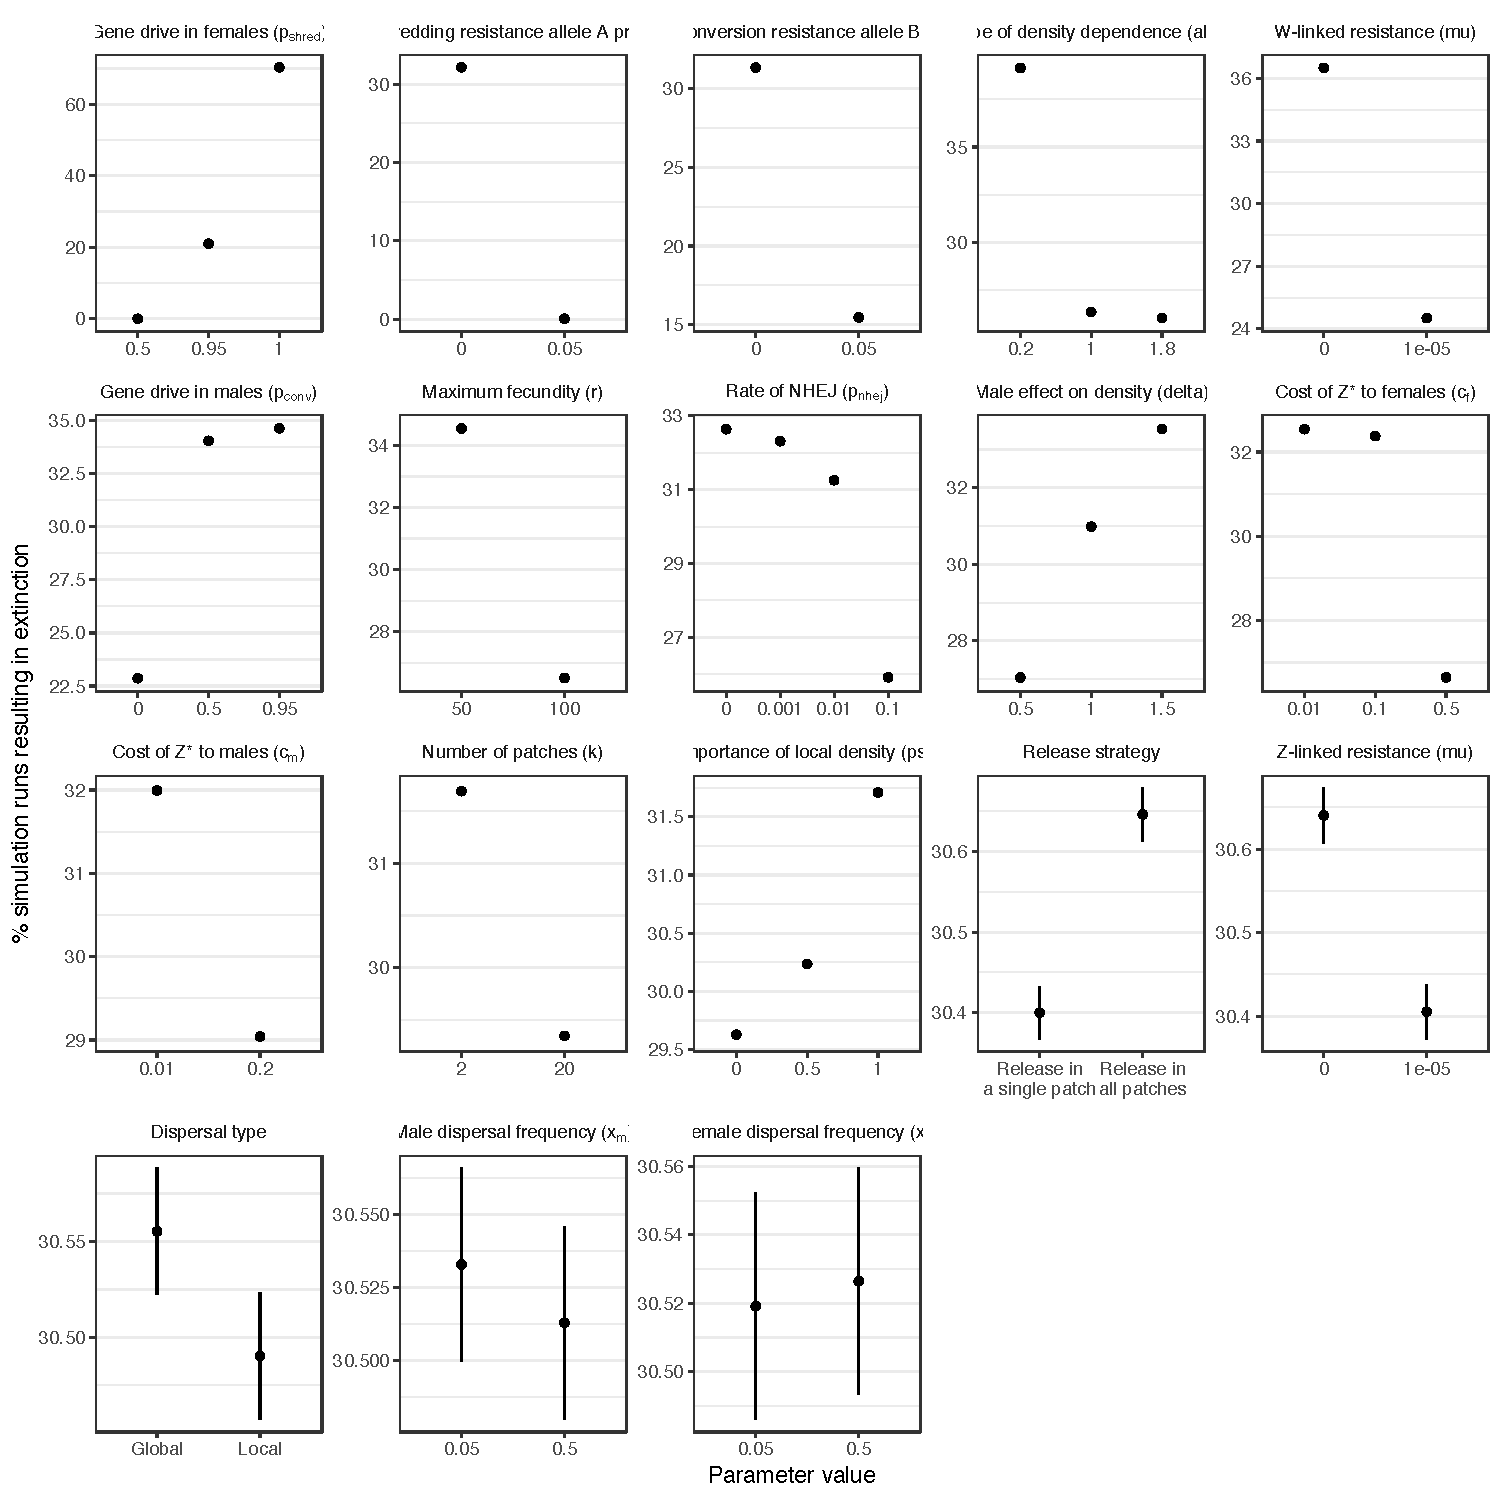
\includegraphics[width=1.0\textwidth]{../figures/figure2.pdf}
\caption{\footnotesize{Three illustrative runs of the simulation, showing evolution in response to the introduction of 20 males carrying a \textit{W}-shredder at Generation 50 (dotted line). In panel A, the driving $Z^*$ allele fixed very quickly, causing population extinction through a shortage of females. In panel B, the $Z^*$ allele spread until its fitness costs began to negate its transmission advantage, causing the population to persist at a reduced size. In panel C, the $Z^*$ allele invaded, which selected for the resistance alleles \textit{A} and $Z^r$ and caused $Z^*$ to go extinct. The population size \textit{N} is shown as a fraction of its maximum value of 10,000. Table S3 gives the parameter spaces used for these three runs.}}
\end{figure}
\newpage

\begin{figure}[h]
\centering
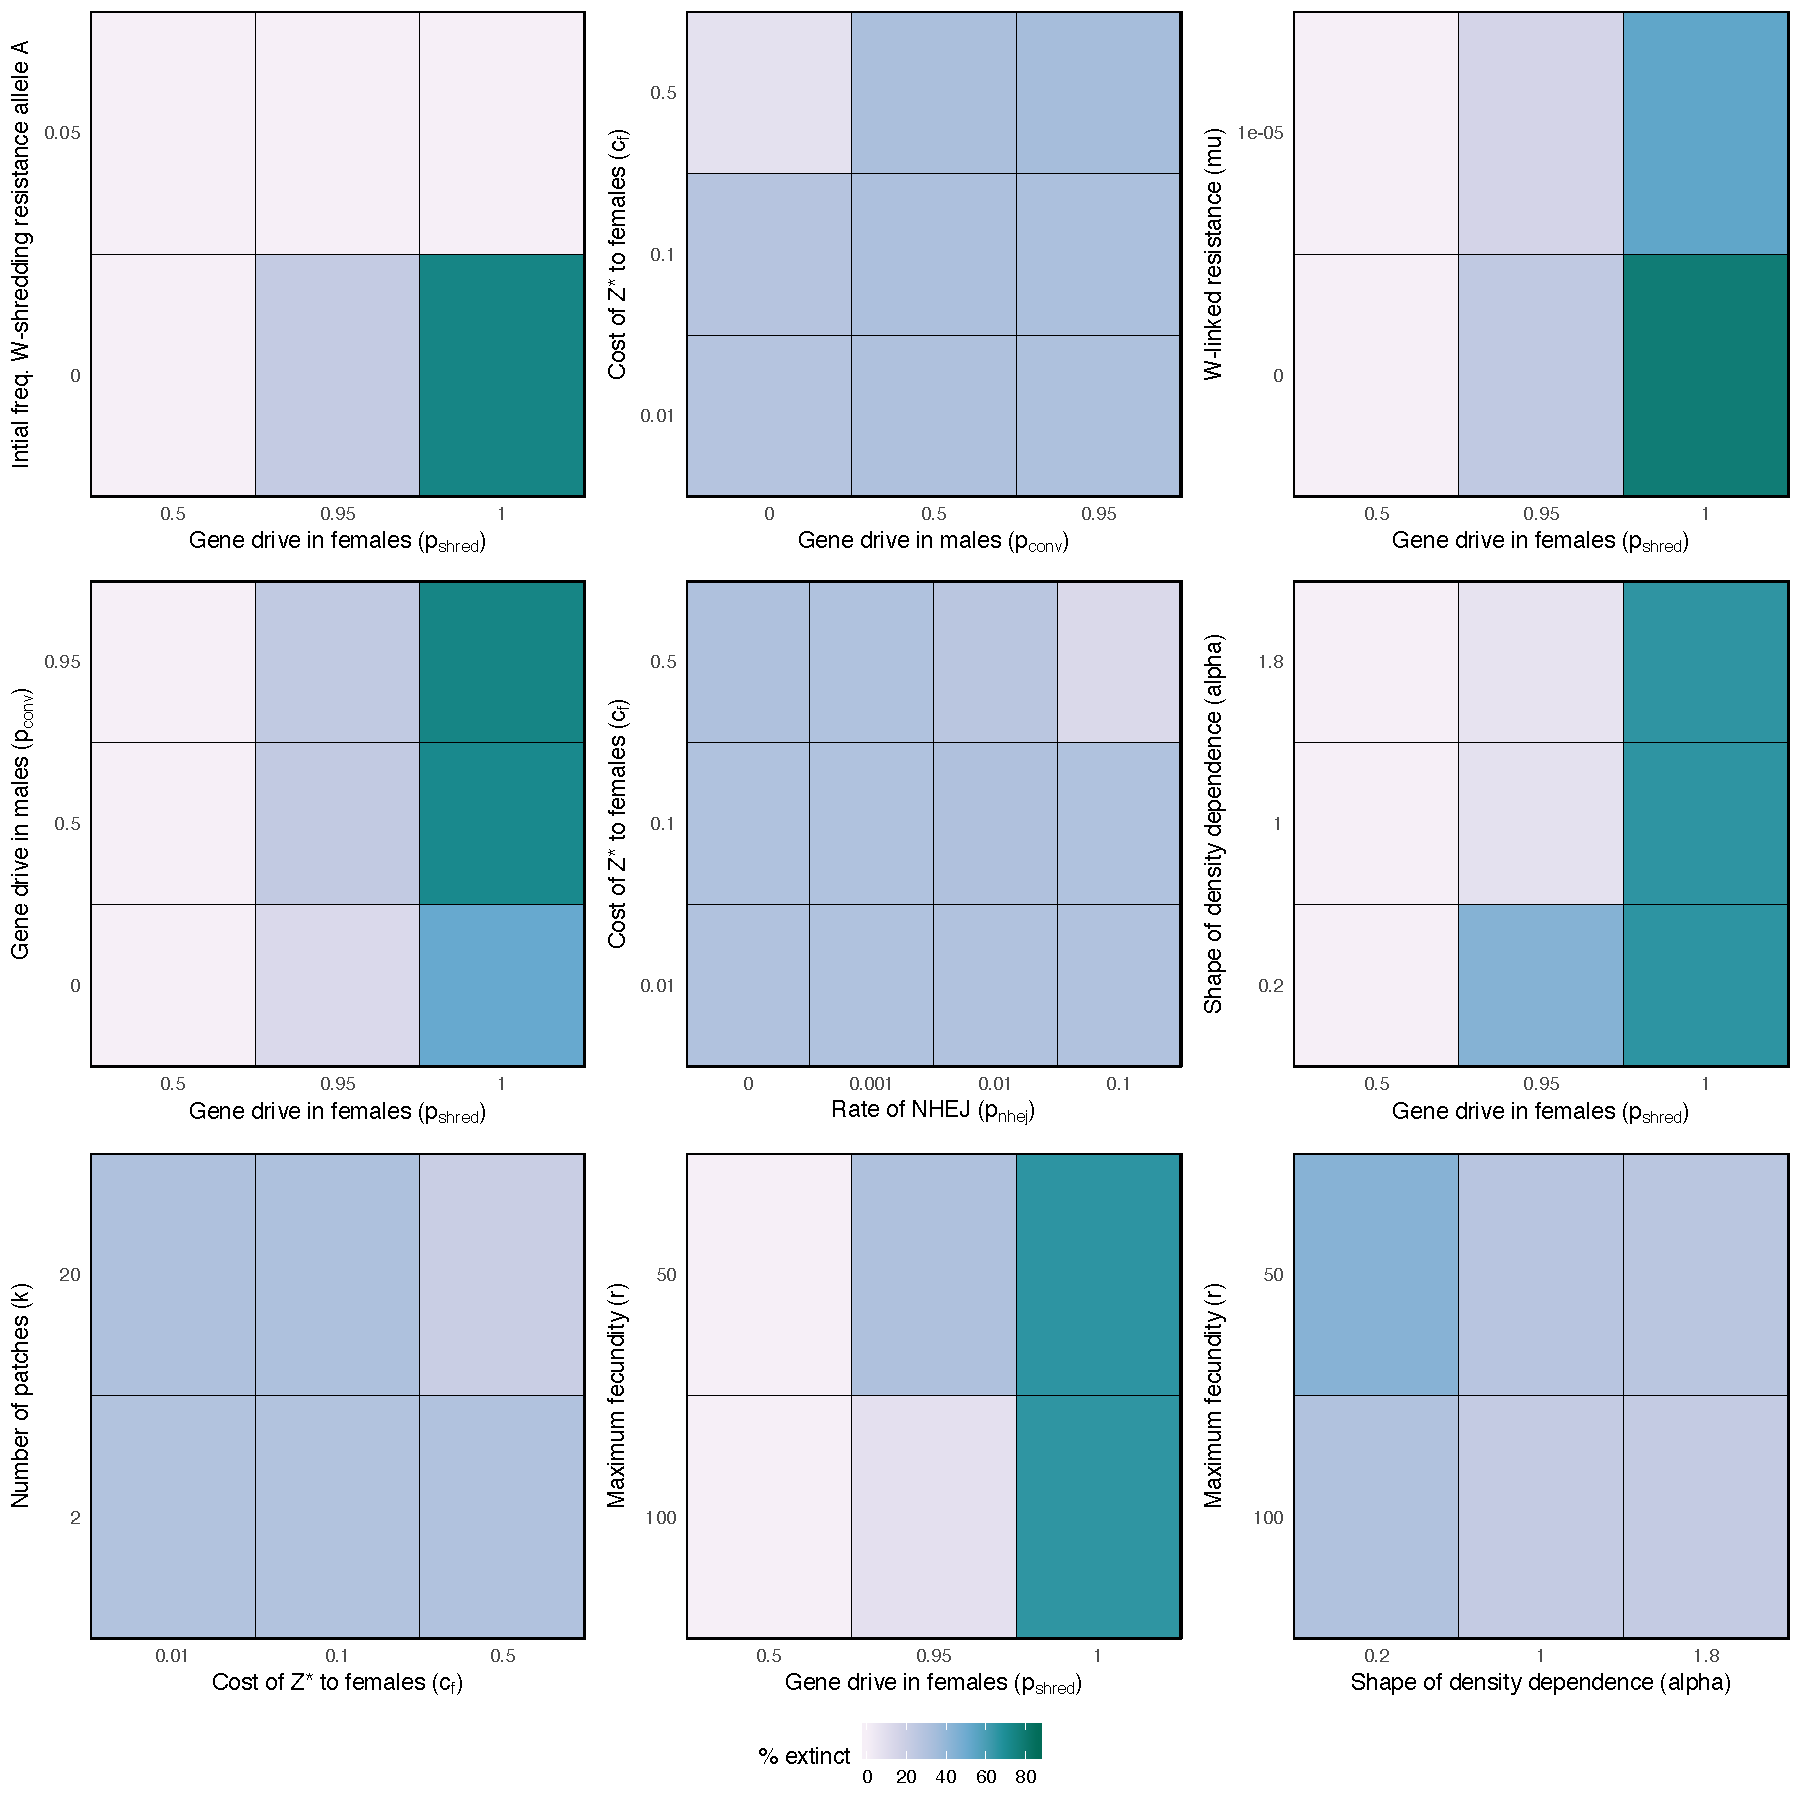
\includegraphics[width=1.0\textwidth]{../figures/figure3.pdf}
\caption{\footnotesize{The percentage of simulations of a \textit{W}-shredder that ended in extinction, for all runs with a particular value (shown on the \textit{x}-axis) for a given parameter (shown in the panels). For example, there were no extinctions in any of the thousands of runs for which I assumed $p_{shred} = 0.5$, while 60\% of runs where $p_{shred} = 1$ resulted in extinction. The panels are ordered by the range of the \textit{x}-axis, which indicates the relative importance of each variable to extinction probability. Figure S3 gives a similar plot for simulations of a female-sterilising $Z^*$ allele.}}
\end{figure}
\newpage

\begin{figure}[h]
\centering
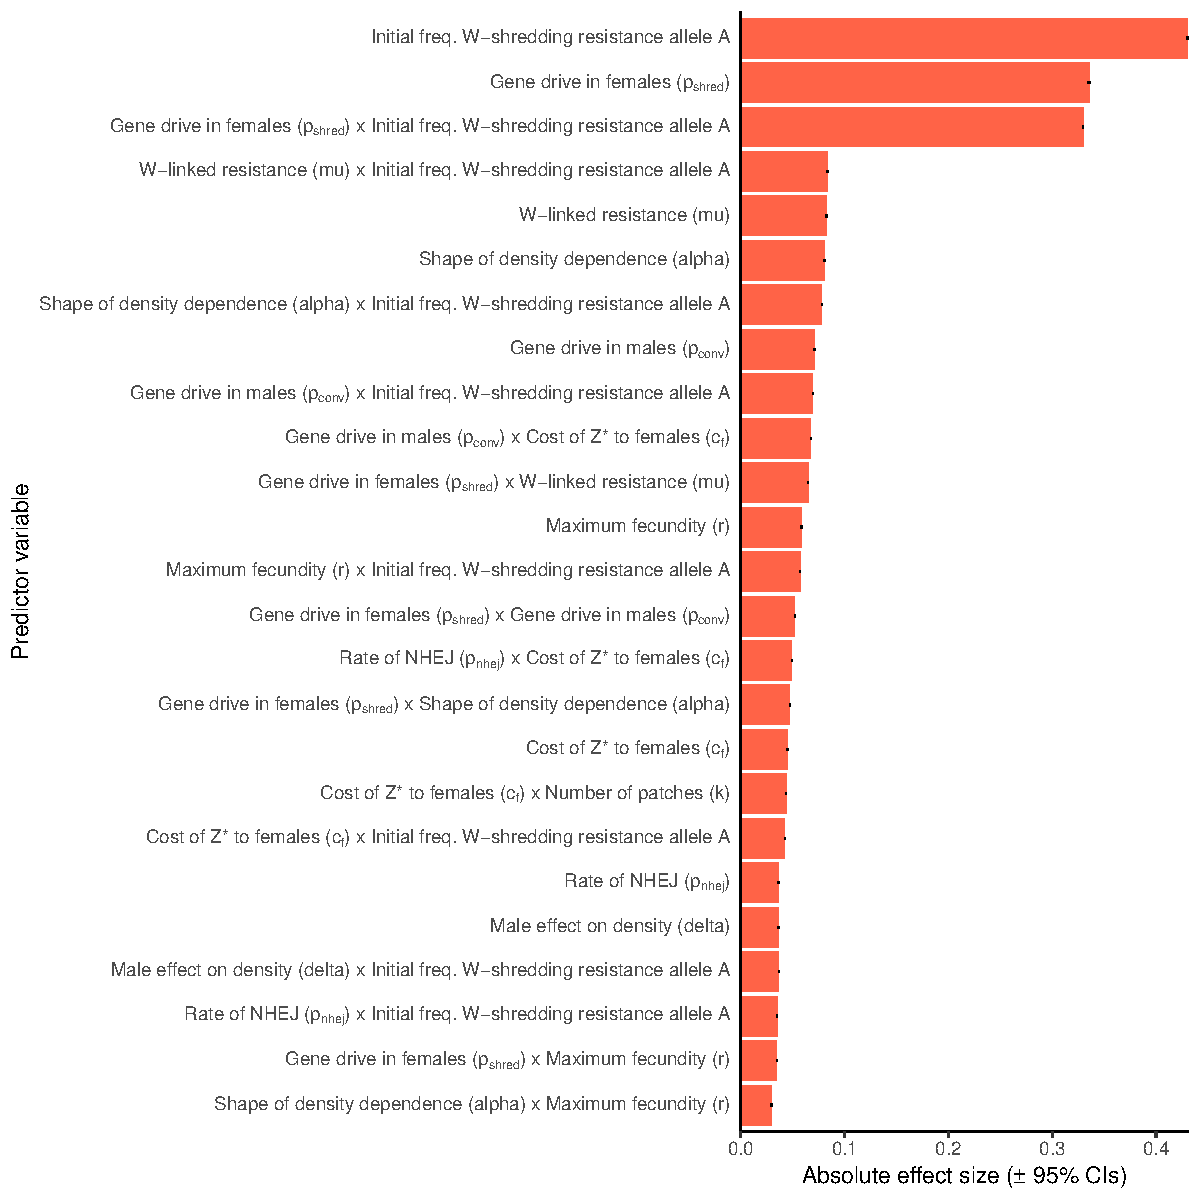
\includegraphics[width=1.0\textwidth]{../figures/figure4.pdf}
\caption{\footnotesize{Relative parameter importance in the simulations of \textit{W}-shredders, for the top 25 most important main effects or two-way interactions (from a binomial GLM that included all the main effects and all their two-way interactions). Each predictor variable was scaled before running the model, meaning that the absolute effect size indicates how important each parameter is to the extinction probability, given the range of values plotted in Figure 3. Figure S5 gives a similar plot for simulations of a female-sterilising $Z^*$ allele.}}
\end{figure}


\dataccess{A website presenting all R scripts used to the run the simulation and
analyse the data can be found at
\url{https://lukeholman.github.io/W_shredder/}.}

\aucontribute{LH performed the analyses and wrote the manuscript.}

\competing{The author declares no conflict of interest.}

\funding{This project was stimulated by an ESEB \emph{Progress Meetings in
Evolutionary Biology} meeting, funded by grants from ESEB (European
Society for Evolutionary Biology) and from the Swiss National Science
Foundation.}


\ack{I thank the organisers (Anna Lindholm and Tom Price), funding bodies
(European Society for Evolutionary Biology; Swiss National Science
Foundation), and attendees of the 2018 ESEB \emph{Progress Meetings in
Evolutionary Biology}, which provided the impetus for this paper. I also
thank Kevin Esvelt and colleagues for describing their ongoing research
on a personal webpage; their ideas greatly influenced this paper.}

\bibliographystyle{RS}
\bibliography{references.bib}


\end{document}
